\chapter{Przegląd istniejących rozwiązań}
\label{cha:rozdzial3}

\section{Wstęp}

Istnieje wiele podejść do zagadnienia jakim jest strumieniowanie danych. Najbardziej popularnym spośród opisywanych poniżej jest para protokołów: Real-time Transport Protocol~i RTP Control Protocol~\cite{RFC3550}. W niniejszym rozdziale opisane zostaną również protokoły: Transmission Control Protocol~\cite{RFC793}, Datagram Congestion Control Protocol~\cite{RFC4340} oraz standard DASH-MPEG~\cite{ISO-IEC-DASH}. W każdym z powyższych przypadków zostną zaprezentowane metody pozwalające na adaptację tych protokołów/standardów do warunków panujących w sieci.

\section{Transmission Control Protocol}

TCP jest protokołem o charakterze połączeniowym mającym sporo zastosowań. Należy do warstwy transportowej modelu ISO/OSI i jest wykorzystywany podczas wymiany poczty elektronicznej (SMTP, IMAP), przeglądania stron internetowych (HTTP, HTTPS), transferu plików (FTP) oraz pozwala na zdalny dostęp do zasobów (SSH)~\cite{Stevens}. Oferuje dostarczanie informacji w sposób niezawodny; sprawdza dane pod względem poprawności (sumy kontrolne) oraz kolejności (numery sekwencyjne)~\cite{RFC793}.

Protokół TCP jest ukierunkowany na niezawodne i bezbłędne dostarczanie danych, co w pewnych przypadkach może powodować opóźnienia. Z tego powodu UDP (w połączeniu z RTP) jest uważane za lepszy wybór przy strumieniowaniu interaktywnych danych multimedialnych. 

Mechanizmy kontroli przeciążeń i przepływu w TCP pozwalają strumieniom na szybkie dostosowanie się do zmienijących się warunków w sieci (zmiennej dostępnej przepustowości). Do regulacji wielkości strumieni wykorzystywane jest okno. Okno jest mechanizmem określającym jak wiele danych można wysłać bez otrzymania potwierdzeń odbioru. Wielkość okna TCP \textit{W} jest obliczna w sposób następujący~\cite{Stevens}:
\begin{center}
$W = min(cwnd, awnd)$
\end{center}
gdzie: 
\begin{itemize}
\item \textit{cwnd (congestion window)} - wielkość okna obliczona na podstawie obciążenia sieci,
\item \textit{awnd (advertised window)} - wielkość okna obliczona na podstawie obciążenia odbiorcy (przesyłana w komunikatach \textit{window update},
\end{itemize}

Kontrola przepływu zapobiega przeciążeniu odbiorcy i może być oparta na regualcji wielkości okna TCP lub na ustaleniu górnej dopuszczalnej przepustowości dla stacji wysyłającej dane.  Stacja odbierająca może zmieniać wielkość okna stacji wysyłającej za pomocą wiadomości \textit{window update}~\cite{Stevens}. Jeżeli stacja odbiorcza nie nadąża z przetwarzaniem pakietów, może zmniejszych wielkość okna ogłaszną w wiadomościach do wysyłającego. Zmniejszenie okna będzie równoznaczne ze spowolnieniem stacji wysyłającej - zmniejszona zostanie ilość pakietów, które można wysłać nie otrzymując ich potwierdzeń odbioru.

Kontrola przeciążeń zapobiega nadmiernemu zalaniu pakietami sieci znajdującej się pomiędzy stacjami końcowymi. TCP nie wykorzystuje  jawnych metod wykrywania obciążenia sieci. Podstawną do założenia, że sieć może być przeciążona są ginące pakiety. Algorytm Slow Start wykorzystuje utracone pakiety jako wyznacznik obciążenia sieci. 
Jego zadaniem jest wykrycie dostępnej przepustowości bez narażania sieci na przeciążenie. W tym celu przesyła pewną ustaloną ilość segmentów i oczekuje na ich potwierdzenie. Z każdą transmisją zakończoną sukcesem ilość wysyłanych segmentów bez potwierdzania jest zwiększana wykładniczo aż do momentu w którym pakiety zaczną ginąć. Drugi algorytm - Congestion Avoidance - pozwala na wykrycie dodatkowego pasma po fazie powolnego startu. Zachowuje się podobnie jak algorytm Slow Start, ale ilość segmentów jest zwiększana liniowo.~\cite{RFC793}

\section{Datagram Congestion Control Protocol}
\label{sec:DCCP}

Protokół DCCP należy do warstwy transportowej i wspiera dwukierunkowe połączenia typu punkt-punkt. Cechą charakterystyczną tego protokołu jest niezawodne nawiązywanie i zrywanie połączenia oraz negocjacja parametrów połączenia. Sama transmisja oparta jest na przesyłaniu datagramów bez potwierdzeń. DCCP posiada kilka mechanizmów kontroli przeciążeń.

Każdy ze wspieranych przez DCCP mechanizmów kontroli przeciążeń posiada identyfikator CCID (Congestion Control Identifier). W trakcie negocjacji parametrów połączenia stacje końcowe wymieniają posortowaną listę akceptowalnych CCID (od najbardziej pożądanego do najmniej pożądanego), a następnie wybierają mechanizm, którym będą posługiwać się w trakcie transmisji~\cite{RFC5762}. RFC standaryzuje dwa mechanizmy kontroli przeciążeń:
\begin{itemize}
  \item CCID 2 - TCP-like Congestion Control
  \item CCID 3 - TCP-Friendly Rate Control
\end{itemize}
Pozostałe numery CCID (0-1 oraz 4-255) pozostają do tej pory niewykorzystane.

Mechanizm TCP-like Congestion Control korzysta z AIMD (Additive Increase/Multiplicative Decrease). Jeżeli TCP wykorzystuje AIMD to po otrzymaniu każdej poprawnej wiadomości ACK od odbiorcy, nadawca powiększa wielkość \textit{cwnd} (wielkość okna) o $\frac{1}{cwnd}$. W razie utraty pakietów okno jest pomniejszane dwukrotnie~\cite{Stevens}. Omawiany mechanizm zachowuje także liczniki czasu znane z TCP oraz algorytm Slow Start~\cite{RFC2581}. TCP-like Congestion Control powinno być wykorzystywane przez aplikacje w których bardziej preferowane jest maksymalne wykorzystanie łącza od utrzymania stabilnego pasma (np. transfer plików)~\cite{RFC4341}.

TCP-Friendly Rate Control jest mechanizmem uznawanym za niezachłanny przy dzieleniu łącza z~innymi strumieniami o charakterze TCP. Niezachłanność tego mechanizmu oznacza, że wykorzystuje on przepustowość nie większą niż dwukrotna wartość przepustowości, która zostałaby wykorzystana przez TCP w tych samych warunkach. TCP-Friendly Rate Control charakteryzuje się także dużo mniejszą zmiennością wartości przepustowości w czasie w porównaniu do TCP, co sprzyja zastosowaniu DCCP z CCID 3 w strumieniowaniu danych multimedialnych. `Wygładzenie' przepustowości transmisji jest okupione wolniejszą niż w TCP szybkością przystosowywania się strumienia do zmian w dostępnym paśmie~\cite{RFC5348}.


\begin{figure}[h!]
	\centering
		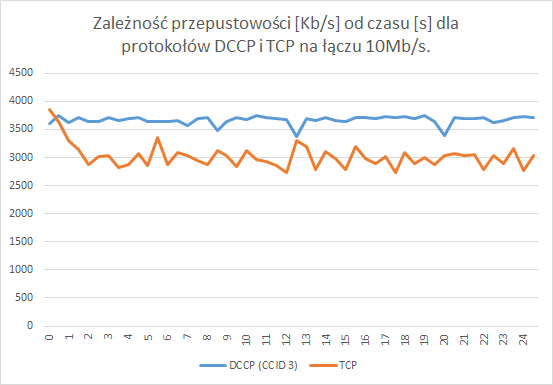
\includegraphics{TCP_DCCP}
	\caption{Wykres zależności przepustowości od czasu dla protokołów TCP i DCCP.}
	\label{TCP_DCCP}
\end{figure}

Rysunek~\ref{TCP_DCCP} przedstawia porównanie działania protokołów TCP i DCCP (CCID 3). W trakcie testu wykorzystano oprogramowanie D-ITG (Distributed Internet Traffic Generator)~\cite{D-ITG}. Test został przeprowadzony z wykorzystaniem dwóch komputerów i przełącznicy Cisco Catalyst 3550 połączonych w~jedną sieć LAN i polegał na jednoczesnym uruchomieniu dwóch strumieni (TCP i DCCP) pomiędzy stacjami końcowymi. Próbkowanie przepustowości przeprowadzono co $0,5s$. Na przełącznicy zaimplementowano politykę pozwalającą na ustalenie przepustowości pomiędzy stacjami na 10Mb/s (zob. Dodatek~A).

\begin{figure}
	\centering
	\begin{tabular}{ l | c | r }
  		Protokół & Średnia przepustowość & Odchylenie Standardowe \\
  		\hline
  		TCP & 3020 Kb/s & 209 \\
  		DCCP (CCID 3) & 3703 Kb/s & 74 \\
	\end{tabular}
	\caption{Tabela porównawcza protokołów TCP i DCCP.}
	\label{TCP_DCCP_table}
\end{figure}

Tabela z rysunku~\ref{TCP_DCCP_table} przedstawia porównanie średniej przepustowości~i odchylenia standardowego dla protokołów TCP i DCCP. Przeprowadzony test potwierdza zachowanie protokołu DCCP (CCID~3) opisane w RFC 5348~\cite{RFC5348}. 

\section{Real-time Transport Protocol i RTP Control Protocol}

RTP (Real-time Transport Protocol) pozwala na transport danych w systemach i aplikacjach czasu rzeczywistego wspierających interaktywne transmisje audio i video. Zwykle wykorzystuje UDP jako protokół transportowy, ale może działać nad innymi protokołami warstwy transportowej modelu ISO/OSI (DCCP, TCP - \cite{RFC3550, RFC5762}). Jeżeli sieć w której działa RTP wspiera multicasting to RTP pozwala na wysłanie danych do wielu odbiorców jednocześnie. RTP nie dostarcza mechanizmów QoS (Quality of Service), ani nie gwarantuje dostarczenia wysłanych danych na czas do odbiorcy.

Protokół RTCP (Real-time Control Protocol) stanowi protokół kontrolny dla RTP. Bazuje na okresowej transmisji pakietów kontrolnych do wszystskich uczestników sesji. Przekazuje informacje od odbiorców do nadawców na temat jakości transmisji. Pakiety RTCP zawierają indentyfikator źródła (Canonical Name) oraz pozwalają na ustalenie liczby uczestników sesji, co pozwala na obliczenie z jaką częstotliwością należy wysyłać pakiety kontrolne.

\begin{figure}[h!]
	\centering
	\begin{tabular}{ l | c | r }
  		Nazwa & Typ & Zalecane pasmo \\
  		\hline
  		GSM & audio & 13 Kb/s \\
  		G728 & audio & 16 Kb/s  \\
  		G729 & audio & 8 Kb/s  \\
	\end{tabular}
	\caption{Przykładowe typy pakietów RTP.}
	\label{RTP_table}
\end{figure}

RTP przenosi dane, które zwykle wymagają ustalonej przepustowości. Dzięki temu prawdopodobieństwo, że strumień RTP będzie systematycznie zajmował coraz większe pasmo jest niewielkie. Z drugiej strony, strumień nie może też zostać ograniczony bez uszczerbku na jakości transmisji danych, szczególnie jeżeli transmisja ma charakter interaktywny. Pasmo potrzebne do sprawnej transmisji zależy od rodzaju przesyłanych danych. Rodzaj przesyłanych danych można identyfikować na podstawie pola Payload Type (zob. rysunek~\ref{RTP_table}) w nagłówku pakietu RTP. Z każdym typem związany jest profil RTP opisujący parametry transmisji (w tym wymaganą przepustowość)~\cite{RFC3551}. Protokół RTP nie posiada odpowiednich mechanizmów kontroli przeciążeń, dlatego powinien korzystać z mechanizmów dostępnych w protokołach niższych warstw (np. DCCP CCID 3).

\section{Podsumowanie}

W powyższym rozdziale opisano kilka podejść do problemu strumieniowania danych multimedialnych. Opisane zostały protokoły TCP, DCCP, RTP/RTCP oraz standard DASH-MPEG. Szczególną uwagę poświęcono mechanizmom adaptacji do zmniennej przepustowości sieci i cechom jakie powinny posiadać protokoły przeznaczone do strumieniowania danych. Do cech tych należą:
\begin{itemize}
\item kontrola przeciążeń i przepływu (TCP)
\item jednostajne wykorzystanie łącza (DCCP CCID3)
\item kanał zwrotny przenoszący informacje na temat sesji (RTCP)
\item możliwość dostosowana parametrów transmisji do warunków w sieci (DASH, TCP)
\end{itemize}

